% ===== UNIT 10: Overview figure + problem formulation (3.1) =====
% Status: AI-DRAFT  (change to REWRITTEN / REVIEWED when done; see CHECKLIST.md)
% Rules: style rewrite only. Keep every \cite, \ref, \label, number, equation and table value as is. Change the wording, not the content.
Figure~\ref{fig:arch} gives the overall architecture of the two-stream
pipeline, from image input through per-stream feature extraction and
post-processing to score-level fusion, together with the two operating points
reported in this paper.

\begin{figure*}[!t]
  \centering
  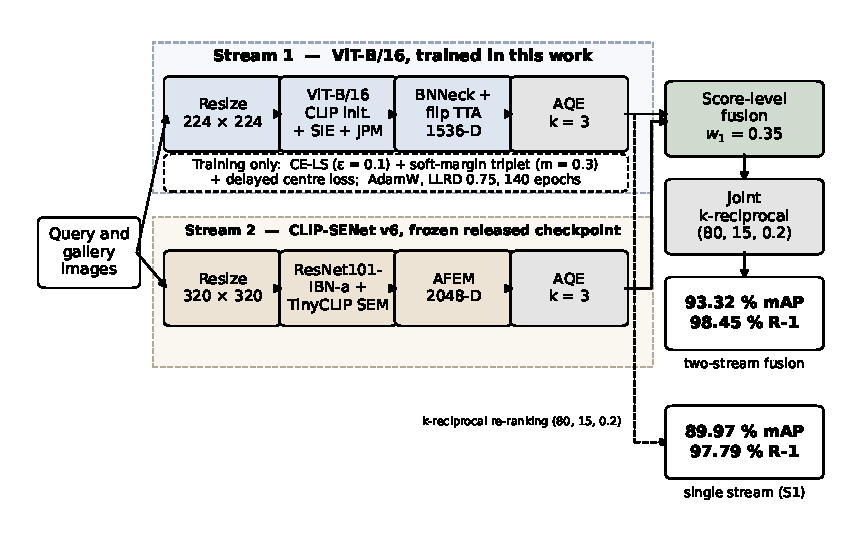
\includegraphics[width=\textwidth]{Fig1}
  \caption{Overview of the two-stream pipeline. Stream~1 (top) is the ViT-B/16
  backbone trained in this work; Stream~2 (bottom) is the frozen, publicly
  released CLIP-SENet v6 checkpoint. Average query expansion is applied to each
  stream, the resulting cosine-similarity matrices are combined by a weighted
  sum, and a single joint $k$-reciprocal re-ranking pass is applied to the
  fused matrix. The dashed path shows the single-stream operating point, in
  which Stream~1 is re-ranked on its own}
  \label{fig:arch}
\end{figure*}

\subsection{Problem formulation}
Given a query image $q$ and a gallery set
$\mathcal{G} = \{g_1, g_2, \ldots, g_N\}$, the task is to retrieve all gallery
images depicting the same vehicle identity as the query and rank them above
non-matching images. Performance is measured by mAP and Rank-1 CMC. The
standard VeRi-776 evaluation protocol~\cite{liu2018provid} employs 1\,678 query
images and 11\,579 gallery images across 200 test identities; training uses
37\,781 images of 576 identities. All reported results strictly follow this
protocol.
